\chapter*{Introduction}
\markboth{\MakeUppercase{Introduction}}{\MakeUppercase{Introduction}}
\addcontentsline{toc}{chapter}{Introduction}

In this project, we are trying to recreate the classic game Snake as it was on the Nokia 3210 mobile phone. We are doing this because we had access to a display from the Nokia 3310 phone, which is roughly the same display.

For the project to work, we need to write drivers for the microcontroller. In this case it will be an ATmega32 from Atmel. We want to try to write reusable drivers that could work with different MCU's with different clock frequencies and so on. These drivers are for interfacing the display and the controller, we are using. 

\begin{figure}
\centering
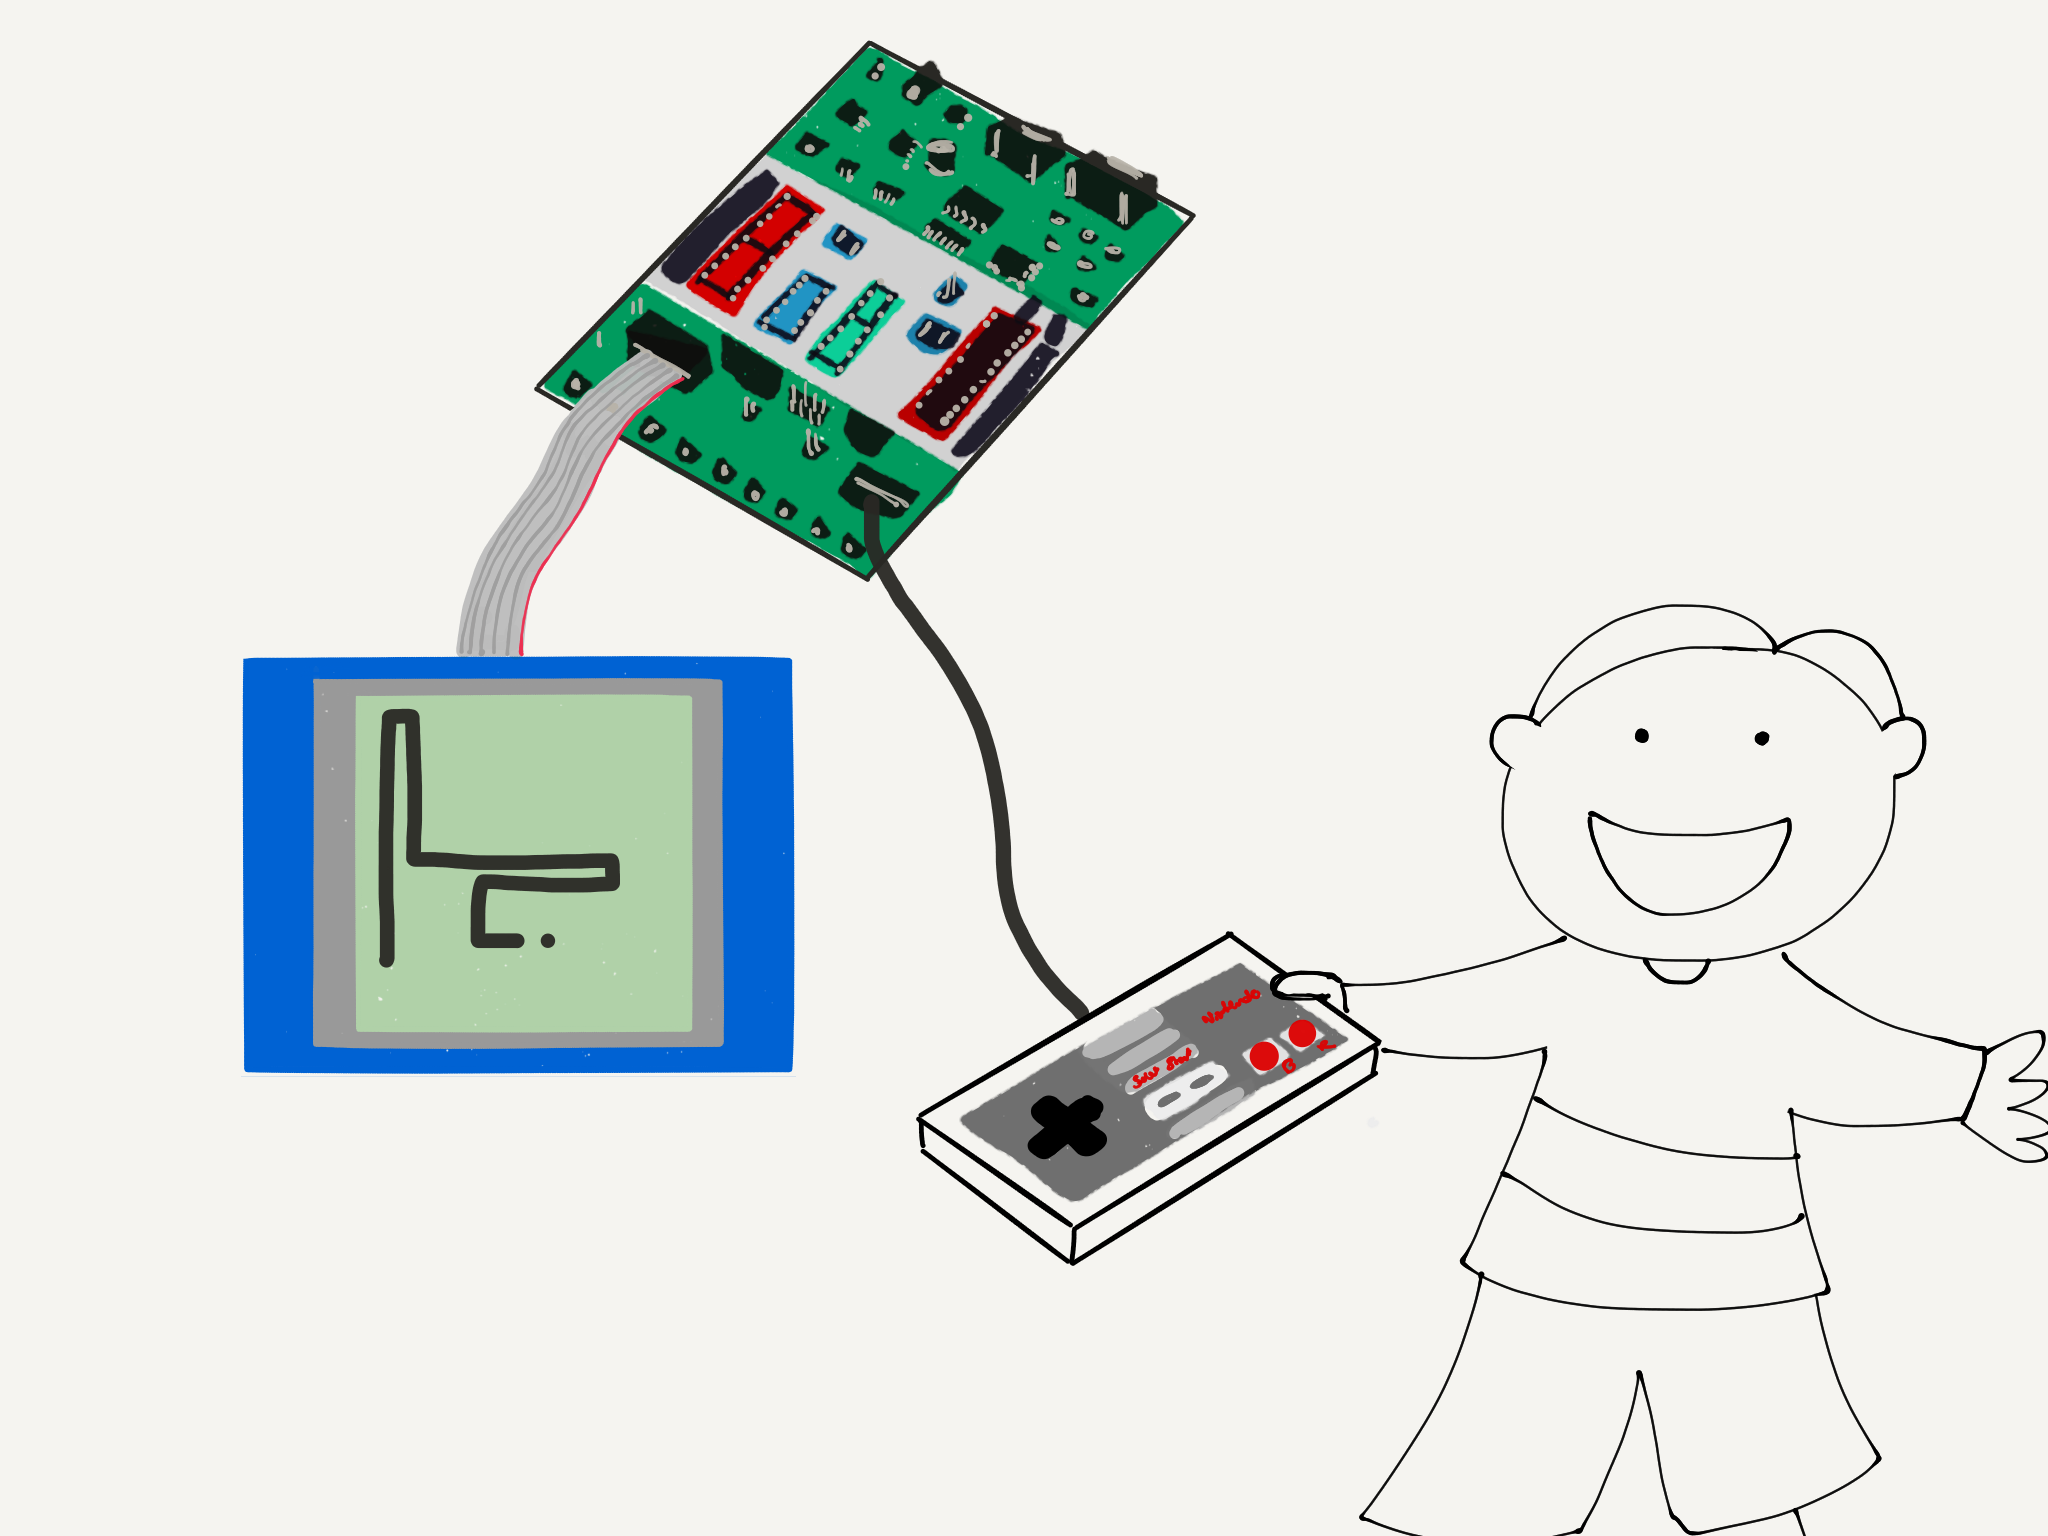
\includegraphics[width=.7\textwidth]{rigebillede.png}
\end{figure}

A large part of the project will be writing the game code. This will be done in C++ as opposed to C. We are doing this because we feel that C++ gives us certain advantages over C like having abstractions via classes.

The game logic for a Snake game is actually quite simple. All you have to do is check for collisions and then move the snake. We, also, need to have win/lose conditions and probably a pause menu. 

The game also has to handle input and output. That means checking the controller for changes and drawing game state to the display.

